%%%%%%%%%%%%%%%%%%%%%%%%%%%%%%%%%%%%%%%%%%%%%%%%%%%%%%%%%%%%%%%%%%%%%%%%%%%%
% AGUJournalTemplate.tex: this template file is for articles formatted with LaTeX
%
% This file includes commands and instructions
% given in the order necessary to produce a final output that will
% satisfy AGU requirements, including customized APA reference formatting.
%
% You may copy this file and give it your
% article name, and enter your text.
%
%
% Step 1: Set the \documentclass
%
%

%% To submit your paper:
%\documentclass[draft]{agujournal2019}
%\usepackage{url} 
%\usepackage{graphicx,natbib,overpic,xcolor}
%\usepackage{apacite}
%\bibliographystyle{unsrtnat}
%this package should fix any errors with URLs in refs.
%\usepackage{lineno}
\usepackage{geometry}
\usepackage{picture}
\usepackage[table,xcdraw]{xcolor}  
\usepackage{tikz}
%\usepackage[inline]{trackchanges} %for better track changes. finalnew option will compile document with changes incorporated.
%\usepackage{soul}
%\linenumbers

\documentclass[draft,linenumbers]{agujournal2019}
\usepackage{apacite}
\usepackage{url} %this package should fix any errors with URLs in refs.
\usepackage{enumitem}
\usepackage{amsmath}
\usepackage{overpic}
\usepackage{pict2e}
\usepackage{bm}
%%%%%%%


\draftfalse
\def\Var{{\textrm{Var}}\,}
%% Enter journal name below.
%% Choose from this list of Journals:
%
% JGR: Atmospheres
% JGR: Biogeosciences
% JGR: Earth Surface
% JGR: Oceans
% JGR: Planets
% JGR: Solid Earth
% JGR: Space Physics
% Global Biogeochemical Cycles
% Geophysical Research Letters
% Paleoceanography and Paleoclimatology
% Radio Science
% Reviews of Geophysics
% Tectonics
% Space Weather
% Water Resources Research
% Geochemistry, Geophysics, Geosystems
% Journal of Advances in Modeling Earth Systems (JAMES)
% Earth's Future
% Earth and Space Science
% Geohealth
%
% ie, \journalname{Water Resources Research}

\journalname{Nature Geoscience}


\begin{document}

%% ------------------------------------------------------------------------ %%
%  Title
%
% (A title should be specific, informative, and brief. Use
% abbreviations only if they are defined in the abstract. Titles that
% start with general keywords then specific terms are optimized in
% searches)
%
%% ------------------------------------------------------------------------ %%

% Example: \title{This is a test title}

\title{Diurnal Self-Aggregation}

%% ------------------------------------------------------------------------ %%
%
%  AUTHORS AND AFFILIATIONS
%
%% ------------------------------------------------------------------------ %%

% Authors are individuals who have significantly contributed to the
% research and preparation of the article. Group authors are allowed, if
% each author in the group is separately identified in an appendix.)

% List authors by first name or initial followed by last name and
% separated by commas. Use \affil{} to number affiliations, and
% \thanks{} for author notes.
% Additional author notes should be indicated with \thanks{} (for
% example, for current addresses).

% Example: \authors{A. B. Author\affil{1}\thanks{Current address, Antartica}, B. C. Author\affil{2,3}, and D. E.
% Author\affil{3,4}\thanks{Also funded by Monsanto.}}

\authors{Jan O. Haerter}


% \affiliation{1}{First Affiliation}
% \affiliation{2}{Second Affiliation}
% \affiliation{3}{Third Affiliation}
% \affiliation{4}{Fourth Affiliation}

\affiliation{1}{Niels Bohr Institute, University of Copenhagen, Blegdamsvej 17, 2100 Copenhagen, Denmark}
%(repeat as many times as is necessary)

%% Corresponding Author:
% Corresponding author mailing address and e-mail address:

% (include name and email addresses of the corresponding author.  More
% than one corresponding author is allowed in this LaTeX file and for
% publication; but only one corresponding author is allowed in our
% editorial system.)

% Example: \correspondingauthor{First and Last Name}{email@address.edu}

\correspondingauthor{Jan O. Haerter}{haerter@nbi.ku.dk}

%% Keypoints, final entry on title page.

%  List up to three key points (at least one is required)
%  Key Points summarize the main points and conclusions of the article
%  Each must be 100 characters or less with no special characters or punctuation and must be complete sentences

% Example:
% \begin{keypoints}
% \item	List up to three key points (at least one is required)
% \item	Key Points summarize the main points and conclusions of the article
% \item	Each must be 100 characters or less with no special characters or punctuation and must be complete sentences
% \end{keypoints}

%\begin{keypoints}
%\item Self-aggregation is possible within short timeperiods, when boundary conditions oscillate,
%\item the effect is nearly independent of domain size or resolution,
%\item the effect requires only moderate temperature amplitudes.
%\end{keypoints}

%% ------------------------------------------------------------------------ %%
%
%  ABSTRACT and PLAIN LANGUAGE SUMMARY
%
% A good Abstract will begin with a short description of the problem
% being addressed, briefly describe the new data or analyses, then
% briefly states the main conclusion(s) and how they are supported and
% uncertainties.

% The Plain Language Summary should be written for a broad audience,
% including journalists and the science-interested public, that will not have 
% a background in your field.
%
% A Plain Language Summary is required in GRL, JGR: Planets, JGR: Biogeosciences,
% JGR: Oceans, G-Cubed, Reviews of Geophysics, and JAMES.
% see http://sharingscience.agu.org/creating-plain-language-summary/)
%
%% ------------------------------------------------------------------------ %%

%% \begin{abstract} starts the second page

%\begin{abstract}
\noindent
{\bf Convective self-aggregation is a paradigm for tropical oceanic cloud organization \cite{wing2017convective} and has been shown to give rise to cloud clusters over timescales of weeks \cite{khairoutdinov2010aggregation,muller2012detailed}.
In contrast to the standard radiative convective equilibrium setup \cite{held1993radiative,tompkins1998radiative}, where surface conditions are held constant, we here allow surface conditions to oscillate diurnally.
%, leading to a repetitive synoptic state, termed perpetual equilibrium \cite{schlemmer2011diurnal,haerter2018intensified}.
While the atmosphere gradually equilibrates at the system scale and domain mean precipitation indeed becomes similar from day to day, the spatial distribution of precipitation is only homogeneous during the first day. 
Already during the second day, the precipitation field is strongly structured and continues to cluster in subsequent days.
The clustering is robust to changes in resolution or domain size, but can be removed by reduction of the amplitude of oscillation, suggesting a transition to organization.
Maximal clustering occurs at scales of $\mathbf{l_{max}\approx 150\;km}$, a scale we relate to the emergence of a convective supercell.
At $\mathbf{l_{max}}$, extreme events are hence likely to be most pronounced and far exceed the rainfall expected at random.
%Our results suggest that a modest diurnal cycle in forcing conditions can lead to aggregation-like structuring of the convective atmosphere.
We explain the transition to clustering using a simple conceptual model, which describes synchronized re-distribution of moisture. 
The results may help clarify, how extremes build up in mid-latitudes and how cloud clustering in the tropics could arise much more rapidly than through conventional self-aggregation alone.
}
%\end{abstract}


%\section{Introduction}\label{sec:intro}
\noindent
As an idealized numerical description of tropical convective self-organization, self-aggregation, where the cloud field segregates into cloudy and less cloudy sub-domains, usually assumes spatially and temporally constant surface moisture (sea surface) and temperature ($\sim 300\;K$) \cite{muller2012detailed}.
It is well-known that many factors influence self-aggregation, such as sea surface temperature and surface feedbacks \cite{hohenegger2016coupled}, domain size, geometry and resolution \cite{muller2015favors}, as well as cold pool effects \cite{jeevanjee2013convective,haerter2019convective}.
Above all, radiation feedbacks have however emerged as the "smoking gun" for sustaining and increasing the inequality between the sub-regions \cite{bretherton2005energy}.
It has been argued, that cloudy regions --- which benefit from warming cloud feedbacks --- tend to emit less heat to space than do cloud-free regions.
Together, these two effects induce net near-surface divergence from cloud-free regions and convergence into already cloudy ones --- bringing more moisture into cloudy regions, thus further enhancing the imbalance.

Whereas numerical simulations assume constant insolation as well as surface boundary conditions, buoy-based instruments do measure diurnal variations in tropical sea surface temperature by typically 0.5-2 K \cite{weller1996surface,johnson1999trimodal} and satellite observations show a diurnal cycle in cloud height for the Madden Julian Oscillation \cite{suzuki2009diurnal,tian2006modulation}.
Diurnal cycles in precipitation also emerge from two-dimensional numerical simulations where variations in insolation are accounted for \cite{liu1998numerical}. 
This and earlier studies\cite{chen1997diurnal} also describe a persistent organized state of a mesoscale convective system, with characteristics of a squall line.
\cite{chen1997diurnal} find a dynamics referred to as "diurnal dancing", which involves a bi-diurnal oscillation of local cloudiness.
\cite{guichard2004modelling,brown2002large,petch2002impact,schlemmer2011diurnal,moseley2016,haerter2018intensified}, as simulated domains show typical build-up on convective available potential energy during the morning hours, and its release in terms of precipitation during the afternoon or evening.
Yet, as the focus was often on the timing or the overall intensity of rainfall, simulated domains were either chosen to be relatively small and model resolutions relatively high. 
State-of-the-art regional climate models now simulate relatively large domains ($\sim 1000$ $km$ at $1$ or $2$ $\;km$ resolution), but include the full complexity of the lateral forcing \cite{ban2015heavy}. 

Sahelian MCS \cite{mathon2001life}
Sea surface impact atmosphere \cite{kawai2007diurnal}
2day equatorial waves \cite{haertel2004dynamics}
scale interaction MJO diurnal cycle \cite{peatman2014propagation}
tropical precipitation extremes and mesoscale systems \cite{rossow2013tropical}
Rich gets richer effect \cite{chou2009evaluating}.
Regular vs. clustered \cite{tompkins2017organization}.


\section{Results}\label{sec:results}
\noindent
We carry out numerical experiments on mesoscale model domains of up to $960\;km\;\times\;960\;km$ and horizontal grid resolutions of $1\;km$, but supplement these by a range of sensitivity experiments ({\it Details:}  Materials and Methods).
We contrast simulations with different amplitudes $T_a$ but equal average surface temperature, and refer to experiments with $T_a=2\;K$ and $5\;K$ as A2 and A5, respectively.
Each numerical experiment is run for several days, allowing for a spin-up and quasi steady state period (Tab.~\ref{tab:experiments} and Fig.~\ref{fig:multi-day_timeseries}). 

\subsection{Domain mean timeseries}
\noindent
Unsurprisingly, the differences in surface temperature amplitudes are reflected in larger amplitudes of near-surface temperatures, $T_{50\;m}$  (Fig.~\ref{fig:domain_mean_timeseries}a and Fig.~\ref{fig:multi-day_timeseries}), but only modest changes to the mean $\overline{T_{50\;m}}$.
Modifications in domain-mean rain are more profound, with $T_a=5\;K$ yielding a relatively sharp single-peak structure, which transitions to a broader and double-peaked structure as $T_a$ is reduced (Fig.~\ref{fig:domain_mean_timeseries}b).
Again, the differences in the temporal mean (dashed lines) are very small.
Approximately proportional curves are found for rain area fraction, which however differ from those of rain rate immediately before the main peak in rate rate (Fig.~\ref{fig:domain_mean_timeseries}c).
These differences are made more transparent when inspecting rain rates conditional on a threshold ($I>I_0$ with $I_0=.5\;mm\;h^{-1}$, Fig.~\ref{fig:domain_mean_timeseries}d). 
Both mean and heavy precipitation show a pronounced evening peak for $T_a=5\;K$ and an early-morning peak for $T_a=2\;K$.
In summary, whereas averages are nearly identical for numerical experiments with varying forcing amplitude, the timeseries of rain rate differ markedly.
Free tropospheric temperatures, which constrain the rate of radiative emission and thereby overall rain rate \cite{Held:2006} are also very similar for the different numerical experiments  (Fig.~\ref{fig:free_trop_temp}).

\subsection{Characterizing the active and quiescent phases}
Now consider the spatial pattern formed by precipitation cells from day to day (Fig.~\ref{fig:daily_mean}). 
During the spin-up from the initial condition, both the $T_a=2\;K$ and $T_a=5\;K$ cases show modest, and relatively homogenous, convective activity throughout the domain. 
During the subsequent model days, convection intensifies for $T_a=2\;K$ because near-surface temperatures gradually increase, but the spatial pattern of events remains rather homogeneous.
In contrast, for $T_a=5\;K$, an inhomogenous pattern organizes, with several locations receiving rather large average rainfall, whereas others remain all but dry. 
In addition, for $T_a=5\;K$, alternations in surface rainfall rate appear to be present, when comparing one day to the next ({\it compare:} Fig.~\ref{fig:daily_mean}e,f).

To quantify spatial inhomogeneities, we track all rain cells and determine their positions ({\it Details:} Materials and Methods).
For each model day of a given experiment, we determine the total number $N$ of track positions.
We then break the horizontal domain area down into square boxes of side length $l$, yielding $n(l)\equiv (L/l)^2$ boxes, and determine the number of tracks falling into each of the boxes.
The probability $p_l$ of a track occurring within one of the boxes at random hence is $p_l=n(l)^{-1}$.
The binomial
\begin{equation}
P_l(m)\equiv {N\choose m}p_l^m\left( 1-p_l \right)^{n-m}
\label{eq:binomial}
\end{equation}
hence describes the probability of $m$ of $n$ randomly distributed tracks falling into one of these boxes during the model day.
The variance of counts $m$ is\cite{feller1957introduction} 
\begin{equation}
\Var_{ran}(l;m) = n\;p_l(1-p_l)
\label{eq:var_ran}
\end{equation}
which we compare to the variance of the empirical data 
\begin{equation}
\Var(l;m) = \sum_{i=1}^{n(l)}(m_i-\langle m\rangle)^2\;,
\label{eq:var_emp}
\end{equation}
where $\langle m\rangle\equiv n\;l/L$ is the average number of tracks per box and the sum in Eq.~\ref{eq:var_emp} is over all boxes $i$.
To compare the empirical to the random variance, we define the clustering index $\mathcal{C}(l)\equiv \Var(l;m)/\Var_{ran}(l;m)$, which is below or above unity, when data are spaced regularly or clustered, respectively.
Results show that, for low amplitudes ($T_a=2\;K$, Fig.~\ref{fig:quantifying_clustering}), $\mathcal{C}(l)<1$ for all box sizes $l$, hence, the spacing of tracks is generally more regular than expected at random.
For larger amplitudes ($T_a=3.5\;K$ and $T_a=5\;K$) regular spacing with $\mathcal{C}(l)<1$ is found only for relatively small box sizes of $l\approx 20\;km$, whereas spacing at larger box sizes is strongly clustered, that is, $\mathcal{C}(l)\gg 1$.
In addition, this clustering increases over time (Fig.~\ref{fig:quantifying_clustering}d).
We can define a box size $l_{max}$, at which $\mathcal{C}(l)$ is maximal.
Despite some noise, $l_{max}\approx 150\;km$ can be identified from the A5 simulation data (Fig.~\ref{fig:quantifying_clustering}e).
We also measure the autocorrelation $c(\tau)$ between day $d$ and $d+\tau$ by computing the Pearson correlation coefficient of daily mean precipitation rates from all grid boxes (Fig.~\ref{fig:quantifying_clustering}f), finding that for all box sizes rainfall is anticorrelated from one day to the next ($c(1)<0$) and positively correlated two days into the future ($c(2)>0$).
Both $c(1)$ and $c(2)$ increase with box size $l$, but appear to level off near $l=200\;km$.


\subsection{Characterizing the dynamics}
What is the cause of this clustering?
To understand this, we consider the dynamics within a given diurnal cycle.
For $T_a=2\;K$, convective rain cells appear at apparently random locations and leave behind a temperature and moisture anomaly [which lasts for x$h$ and y$h$, respectively, measured by the typical decay coefficient.]
For $T_a=5\;K$, the loci of initial rain cell at the rain onset of the second day ($d=2$) already are non-random, with many cells occurring in a relatively small area during almost the same time [quantify spatio-temporal density and compare with low-amplitude case].
[Insert the case study here using a 480x480 simulation, showing an image sequence of the growing supercell and the resulting large cold pool.]
Due to the high density of occurrence, the cold pools resulting from the individual cells cannot dissipate before other cold pools merge with them, forming a conglomerate of cold pools with large negative temperature anomaly, reaching almost to the top of the boundary layer [insert a plot with CP height for both cases on day 2 for 480 x 480].
The resulting merged cold pool spreads outward from the dense region of rain cells and leaves behind a relatively cold and dry subregion.
Conversely, the surrounding of this merged cold pools benefit from the moisture transported by the cold pool and the additional latent heat provided by relatively strong surface fluxes due to the cold pool's strong horizontal winds.

To corroborate this finding, we contrast domain subregions, which receive intense versus weak precipitation during a given model day (Fig.~\ref{fig:moisture_oscillations}).
For each of these subregions, we compute the vertical specific humidity profile, $q_v(z)$, during the early morning and in the evening, that is, before and after the onset of precipitation in A5.
Regions of intense rainfall are characterized by enhanced moisture near cloud base before precipitation onset, but marked depletion after rainfall has occurred.
Conversely, the regions of weak rainfall experience nearly a "mirror image", with depressed moisture before but enhanced values after rainfall.
The bi-diurnal dynamics for A5 can hence be characterized as an oscillation of cloud-base moisture, driven by the lateral expansion of convective supercells.
In A2, these moisture oscillations are all but lacking (Fig.~\ref{fig:moisture_oscillations}d---f), a finding that falls in line with the absence of supercells.

To quantify the effect on cold pools in the cases $T_a=2\;K$ and $T_a=5\;K$, we perform a simple cold pool tracking, using only temperature anomalies as a measure ({\it Details:} Materials and Methods).
We find that, for the lower amplitude, CP mergers are relatively rare and CPs areas remain of modest extent. 
For the large amplitude, CP mergers are ubiquitous and large, long-lived "super-cold pools" are frequently encountered. 
Additionally computing the height of CPs in the two cases, we find that $T_a=5\;K$ gives CPs nearly reaching the level of free convection [make an SI plot here]. 


\subsection{Conceptual model}


\begin{figure*}
\centering
%\begin{overpic}
%\includegraphics[height=0.33\linewidth]{cavities}
\centering
\begin{overpic}[width=0.4\textwidth ]{dummy.pdf}
\put(-57,0){
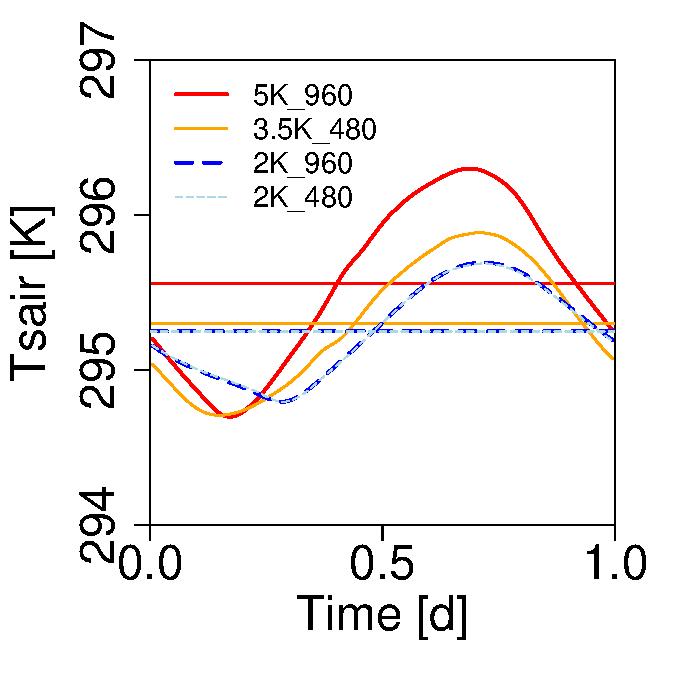
\includegraphics[trim={0 0 0cm 0}, clip, height=0.25\linewidth]{tsair_varying_ampl_timeseries_agg.pdf}}
\put(-15,0){
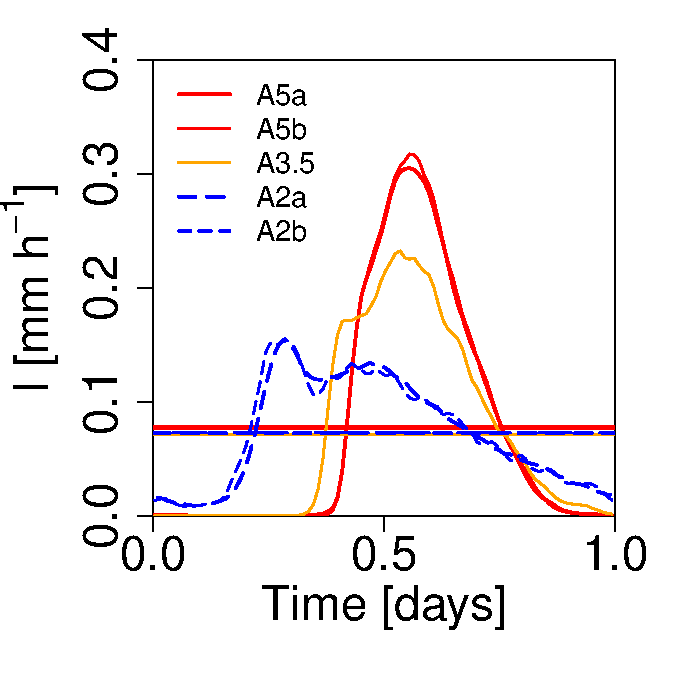
\includegraphics[trim={0 0 0cm 0}, clip, height=0.25\linewidth]{prcp_varying_ampl_timeseries_agg.pdf}}
\put(27,0){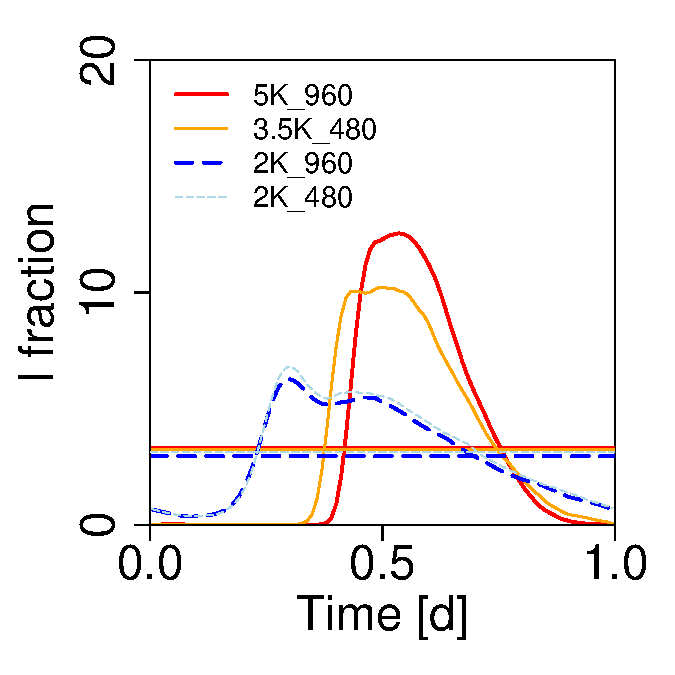
\includegraphics[trim={0 0 0cm 0}, clip, height=0.25\linewidth]{pfrac_varying_ampl_timeseries_agg.pdf}}
\put(69,0){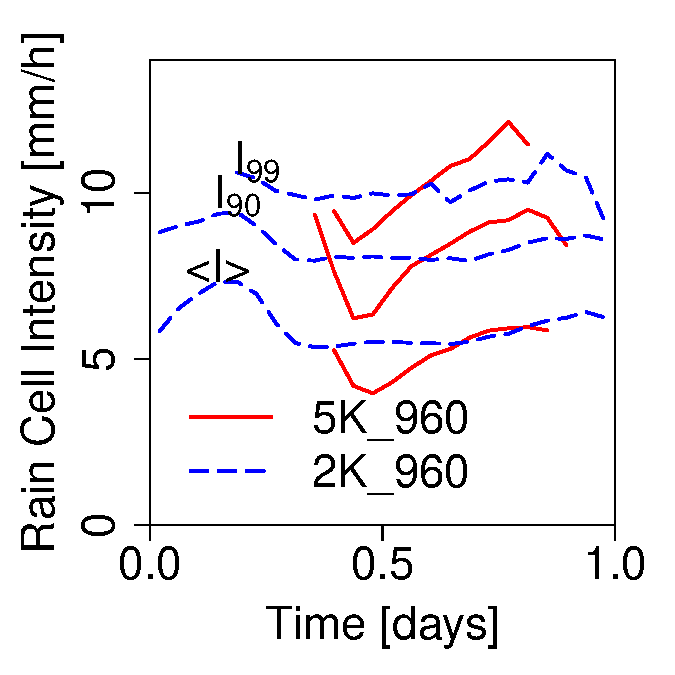
\includegraphics[trim={0 0 0cm 0}, clip, height=0.25\linewidth]{diurnal_heavy_precip.pdf}}
\put(-47,42){\bf a}
\put( -3,42){\bf b}
\put( 38,42){\bf c}
\put( 80,42){\bf d}
\end{overpic}
\caption{{\bf Diurnal cycles of domain averaged quantities}. [here we might also want to show $T(6000m)$ and specific humidity.]
Each quantity was averaged over the spatial model domain. The timeseries is a compound diurnal cycle, where equal times of day were averaged over all available model days.
{\bf a}, Near-surface temperature for simulations with different imposed surface temperature amplitudes, as labeled in legend. Horizontal lines of corresponding colors represent the time average of each simulation.
{\bf b}, Analogous to (a), but for rain intensity.
{\bf c}, Analogous to (a), but for rain area fraction.
{\bf d}, Mean, 90'th and 99'th percentiles of rain intensity for $T_a=5\;K$ and $T_a=2\;K$, as labeled in the panel.
}
\label{fig:domain_mean_timeseries}
\end{figure*}



\begin{figure*}
\centering
\begin{overpic}[width=0.4\textwidth ]{dummy.pdf}
\put(-70,40){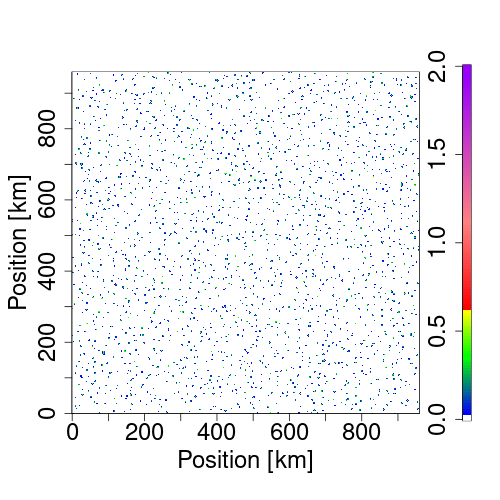
\includegraphics[height=0.38\linewidth,trim=0cm 2.75cm 2.6cm 0cm, clip]{var1_daymean_T0_300K_ampl_4_1km_large_1-96.png}}
\put(0,40){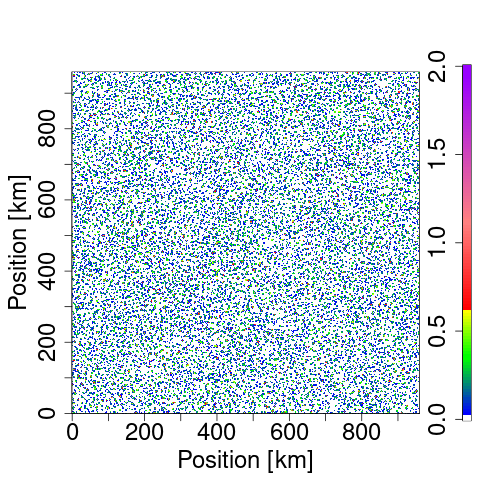
\includegraphics[trim={2.4cm 2.75cm 2.6cm 0cm}, clip, height=0.38\linewidth]{var1_daymean_T0_300K_ampl_4_1km_large_289-384.png}}
\put(60,40){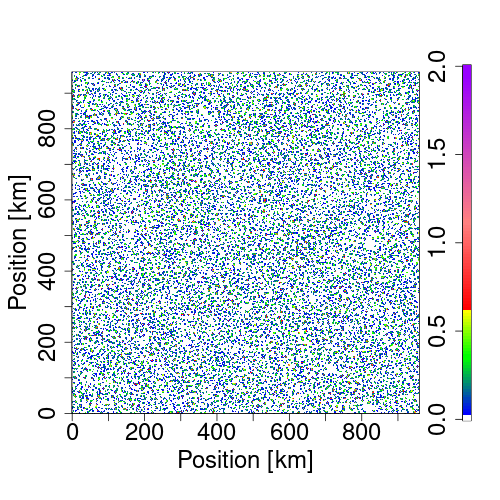
\includegraphics[trim={2.4cm 2.75cm 0cm 0cm}, clip, height=0.38\linewidth]{var1_daymean_T0_300K_ampl_4_1km_large_385-480.png}}
\put(-70,-35){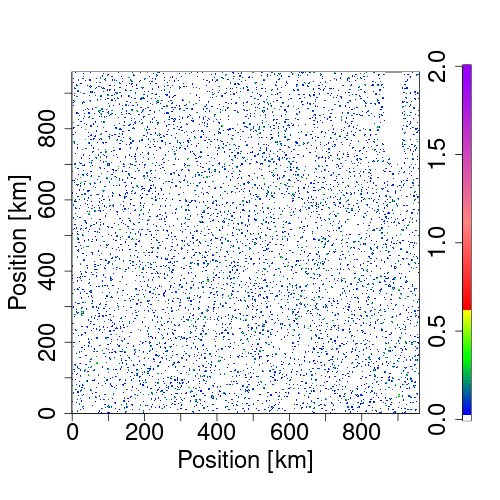
\includegraphics[trim={0cm 0cm 2.6cm 1.75cm}, clip, height=0.4\linewidth]{var1_daymean_T0_300K_ampl_10_1km_large_1-144.png}}
\put(0,-35){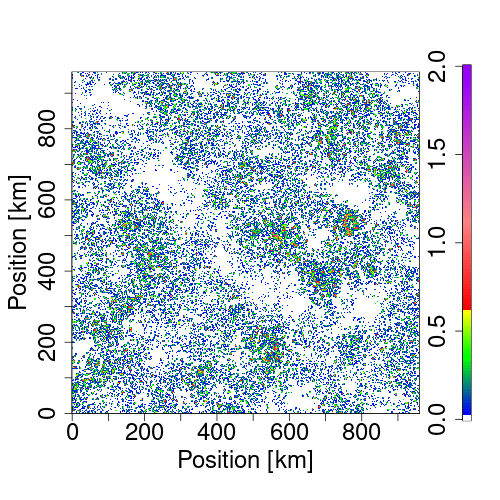
\includegraphics[trim={2.4cm 0cm 2.6cm 1.75cm}, clip, height=0.4\linewidth]{var1_daymean_T0_300K_ampl_10_1km_large_433-576.png}}
\put(60,-35){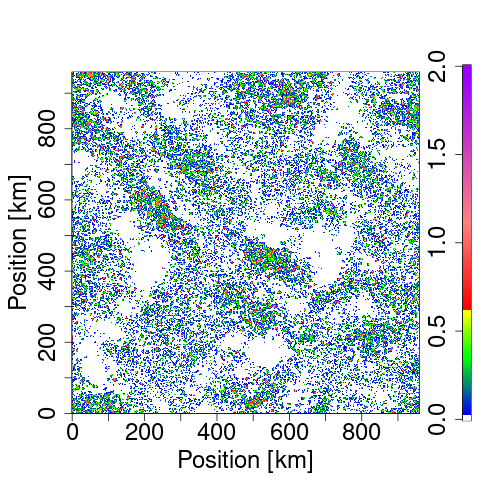
\includegraphics[trim={2.4cm 0cm 2.6cm 1.75cm}, clip, height=0.4\linewidth]{var1_daymean_T0_300K_ampl_10_1km_large_577-720.png}}
\put(-62,97){\large \bf a}
\put(-2,97){\large \bf b}
\put(59,97){\large \bf c}
\put(-62,34){\large \bf d}
\put(-2,34){\large \bf e}
\put(59,34){\large \bf f}

\put(-58,90){\large $T_a=2\;K$}
\put(-58,27){\large $T_a=5\;K$}

\put(5,72){\color{black}\line(0,-1){10}}
\put(5,62){\color{black}\line(1,0){10}}
\put(5,72){\color{black}\line(1,0){10}}
\put(15,72){\color{black}\line(0,-1){10}}

\put(5,10){\color{black}\line(0,-1){10}}
\put(5,0){\color{black}\line(1,0){10}}
\put(5,10){\color{black}\line(1,0){10}}
\put(15,10){\color{black}\line(0,-1){10}}

\put(65,72){\color{black}\line(0,-1){10}}
\put(65,62){\color{black}\line(1,0){10}}
\put(65,72){\color{black}\line(1,0){10}}
\put(75,72){\color{black}\line(0,-1){10}}

\put(65,10){\color{black}\line(0,-1){10}}
\put(65,0){\color{black}\line(1,0){10}}
\put(65,10){\color{black}\line(1,0){10}}
\put(75,10){\color{black}\line(0,-1){10}}

\end{overpic}
%\begin{picture}
%\put(0,15){\circle(20)}
%\end{picture}
\vspace{2cm}
\caption{{\bf Transition to a clustered rainfall state.}
{\bf a}, Surface rainfall average during the first day ($d=1$, spin up) for $\Delta T=2\;K$.
{\bf b}, Similar to (a), but for $d=3$.
{\bf c}, Similar to (a), but for $d=4$.
{\bf d---f}, Similar to (a)---(c), but for $\Delta T=5\;K$.
To highlight the spatial and temporal variation, boxes of side length $l=150\;km$ are shown at equal positions in panels b,c,e,f.
}
\label{fig:daily_mean}
\end{figure*}



\begin{figure}
\centering
\begin{overpic}[width=0.4\textwidth ]{dummy.pdf}
\put(-50,40){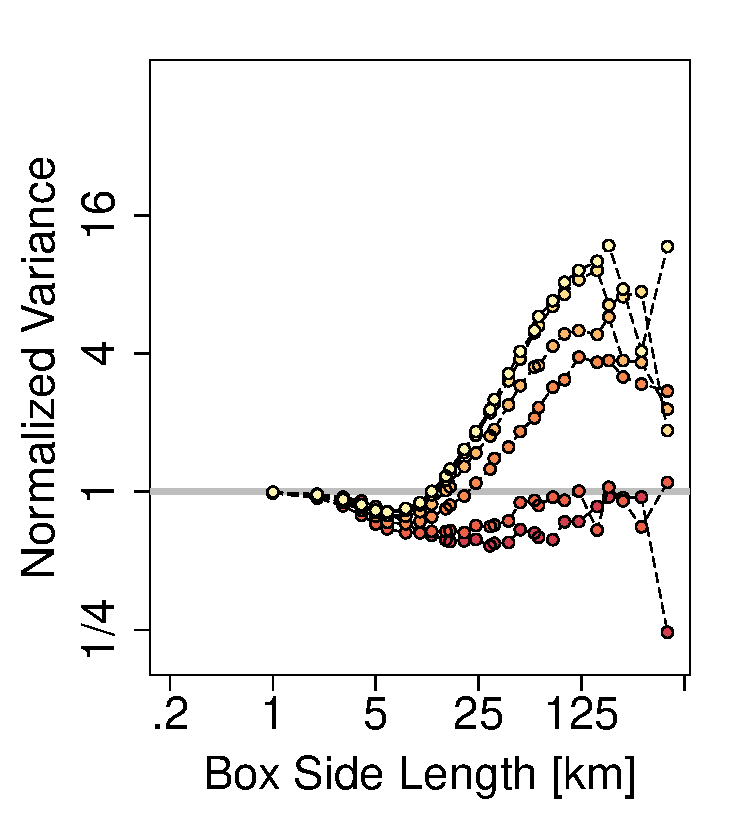
\includegraphics[trim={0cm 0cm 0cm 0cm}, clip, height=0.4\linewidth]{var_5K_960.pdf}}
\put(10,40){\includegraphics[trim={2cm 0cm 0cm 0cm}, clip, height=0.4\linewidth]{{var_3.5K_480}.pdf}}
\put(60,40){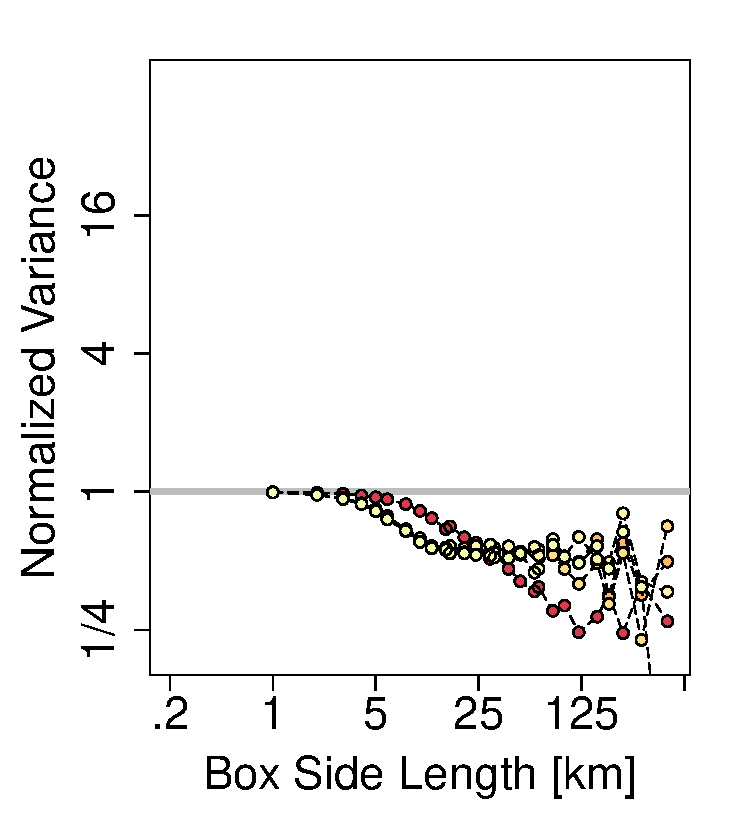
\includegraphics[trim={2cm 0cm 0cm 0cm}, clip, height=0.4\linewidth]{var_2K_960.pdf}}
\put(-50,-25){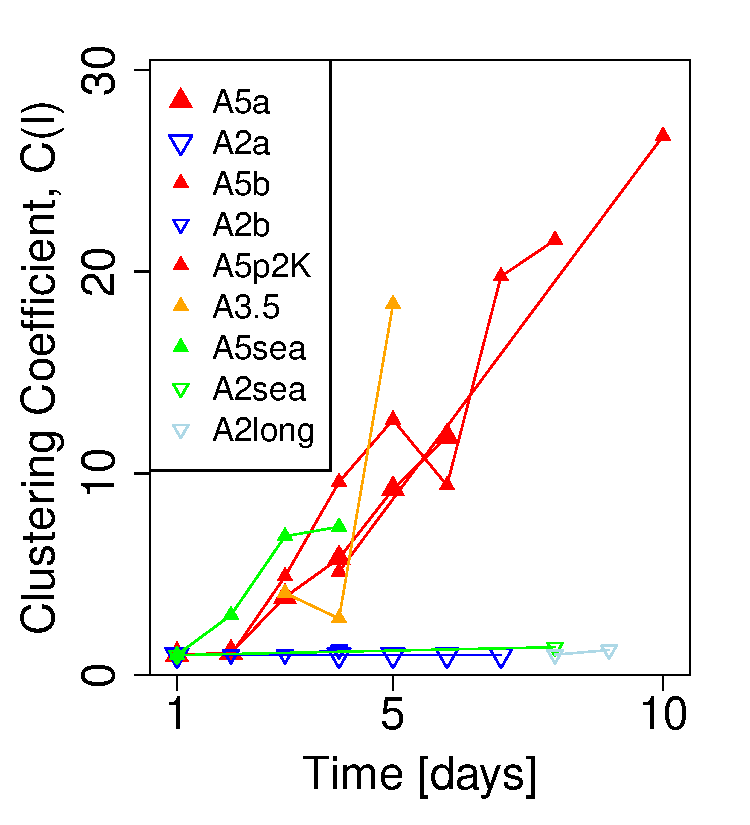
\includegraphics[trim={0cm 0cm 0cm 0cm}, clip, height=0.35\linewidth]{maxvar_vs_day.pdf}}
\put(5,-25){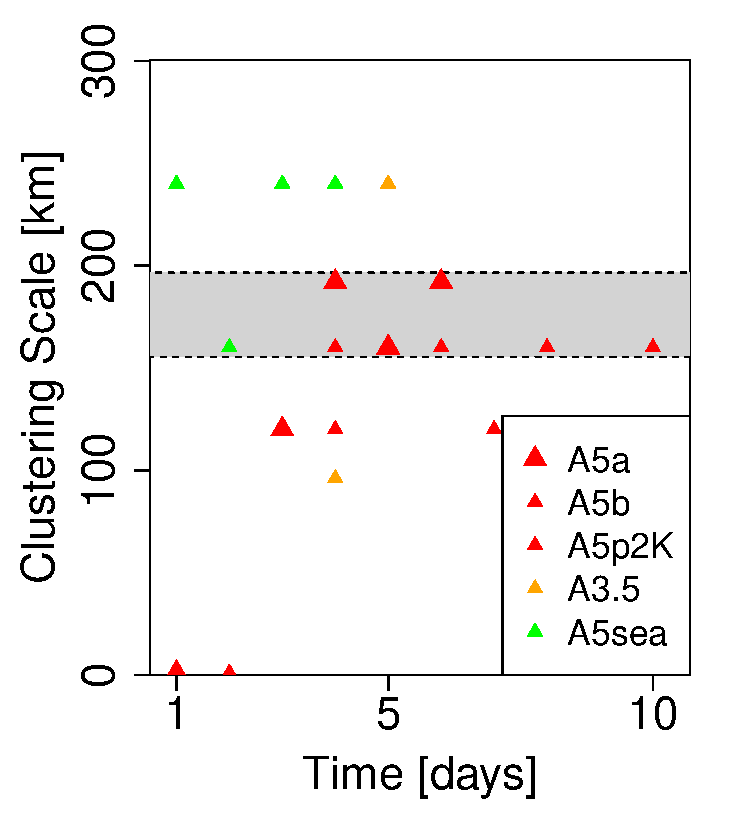
\includegraphics[trim={0cm 0cm 0cm 0cm}, clip, height=0.35\linewidth]{maxvarPos_vs_day.pdf}}
\put(60,-25){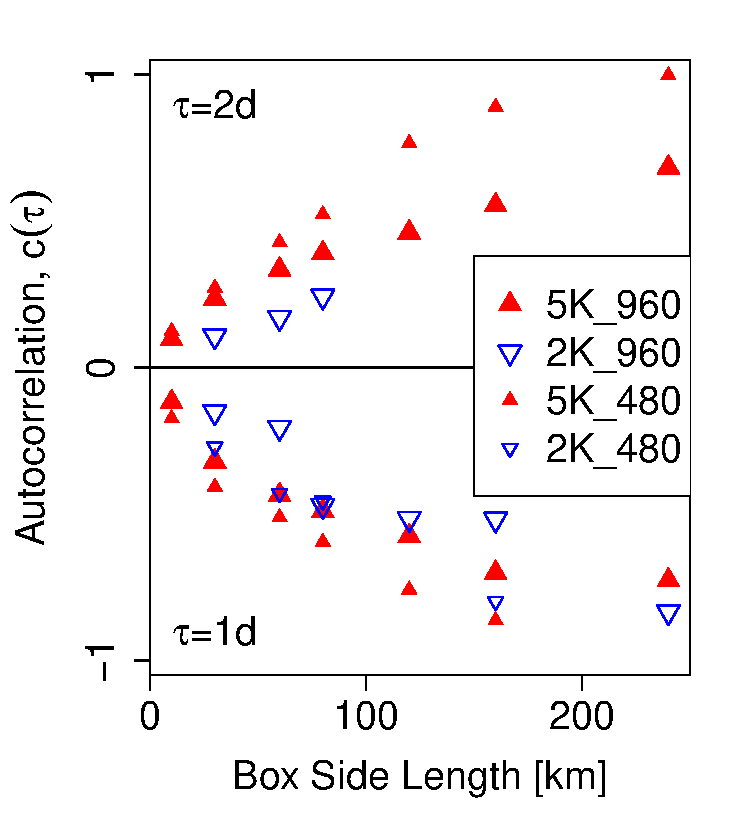
\includegraphics[trim={0cm 0cm 0cm 0cm}, clip, height=0.35\linewidth]{autocor_vs_day.pdf}}
\put(-38,108){\large \bf a}
\put(15,108){\large \bf b}
\put(62,108){\large \bf c}
\put(-40,34){\large \bf d}
\put(15,34){\large \bf e}
\put(70,34){\large \bf f}
\put(-38,100){\large $\Delta T=5\;K$}
\put( 12,100){\large $\Delta T=3.5\;K$}
\put( 62,100){\large $\Delta T=2\;K$}

\end{overpic}
\vspace{2cm}
\caption{{\bf Quantifying clustering using spatial variance.}
{\bf a}, Spatial variance at different box sizes for $\Delta T=5\;K$.
Curves of colors ranging from red to green correspond to increasing days.
Note that at small scales ($\sim 10\;km$) and early times ($<2\;d$) rain events are distributed regularly, while at larger scales ($\sim 150\;km$) and later times, events are clustered.
Note the double-logarithmic axis scaling.
{\bf b}, Analogous to (a), but for $\Delta T=3.5\;K$.
{\bf c}, Analogous to (a), but for $\Delta T=2\;K$. Note that the normalized variance remains in the regular range and does not exceed unity.
{\bf d}, Peaks of variance anomalies vs. time for different simulations [mark them in legend]. 
Note the general increase for large $\Delta T$ but flat behaviour for small $\Delta T$.
{\bf e}, Scales of clustering, i.e. the peak position in all clustered distributions, such as in (a)---(b). [mark the average somehow]. 
{\bf f}, Autocorrelation coefficient $c(\tau)$ for $\tau=1\;d$ and $\tau=2\;d$, showing increasing autocorrelation with scale.
}
\label{fig:quantifying_clustering}
\end{figure}


\begin{figure}
\centering
\begin{overpic}[width=0.4\textwidth]{dummy.pdf}
\put(-55,15){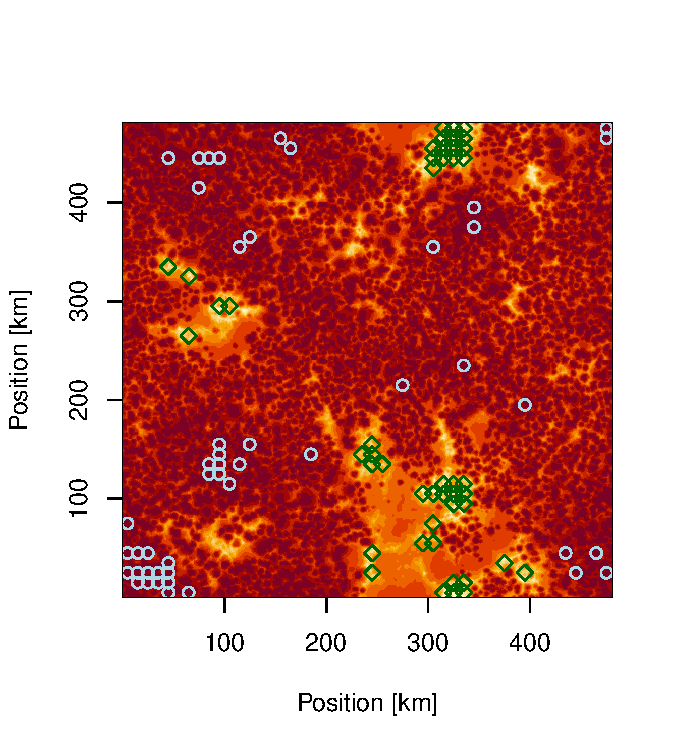
\includegraphics[trim={0cm 2.1cm 0cm 0cm}, clip, height=0.235\linewidth]{T0_300K_ampl_10_1km_1773-20402dPlot_precip_marked_points.pdf}}
\put(-14,16){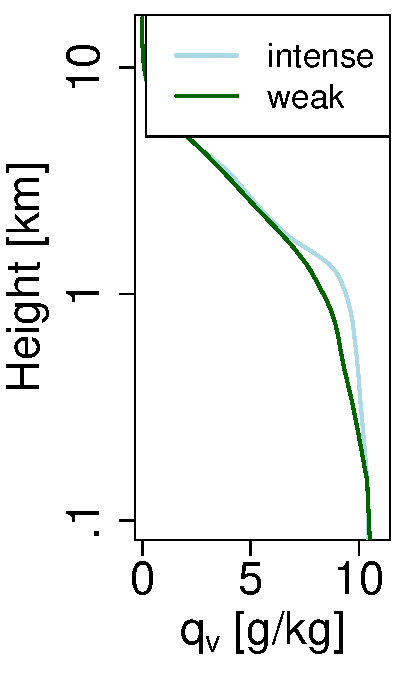
\includegraphics[trim={0cm 2.1cm 0cm 0cm}, clip, height=0.19\linewidth]{T0_300K_ampl_10_1km_1773-2040_comparison_q_17.pdf}}
\put(10,16){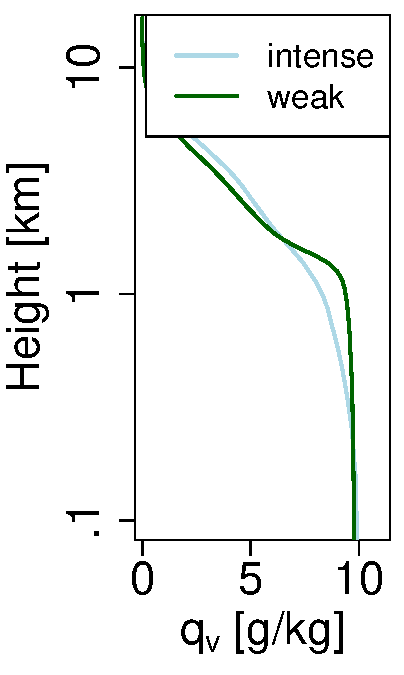
\includegraphics[trim={2cm 2.1cm 0cm 0cm}, clip, height=0.19\linewidth]{T0_300K_ampl_10_1km_1773-2040_comparison_q_221.pdf}}
\put(-55,-30){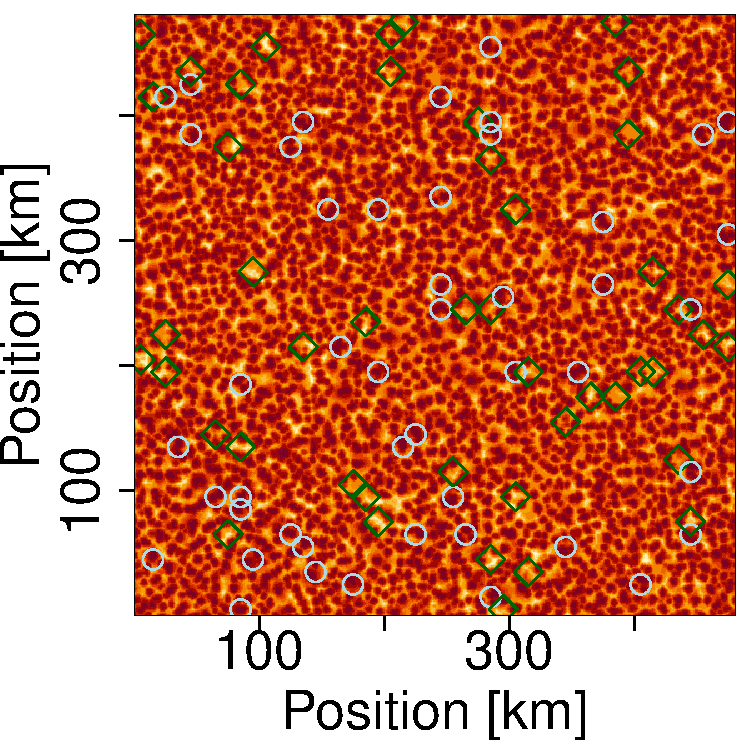
\includegraphics[trim={0cm 0cm 0cm 0cm}, clip, height=0.28\linewidth]{T0_300K_ampl_4_1km_865-11722dPlot_precip_marked_points.pdf}}
\put(-14,-28){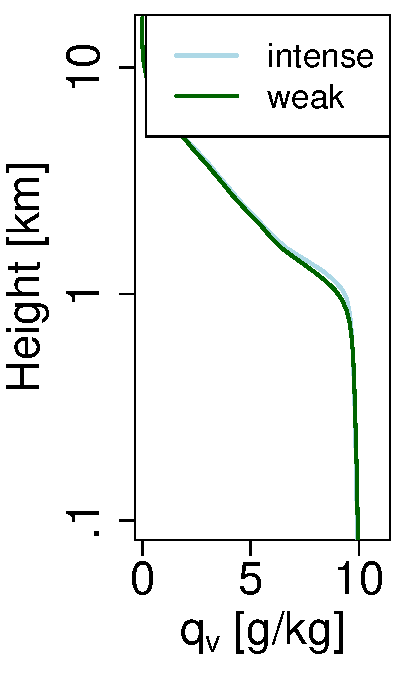
\includegraphics[trim={0cm 0cm 0cm 0cm}, clip, height=0.23\linewidth]{T0_300K_ampl_4_1km_865-1172_comparison_q_1.pdf}}
\put(10,-28){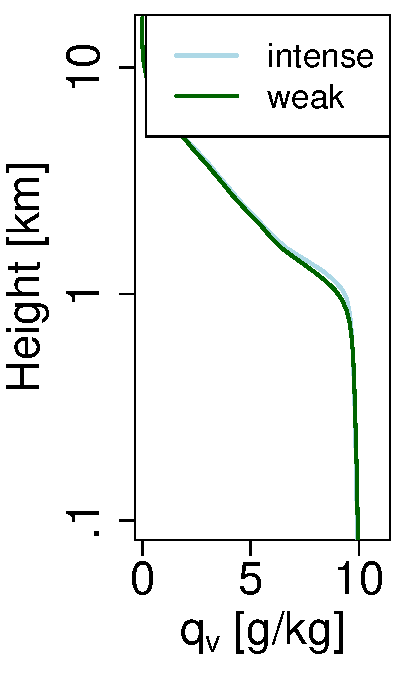
\includegraphics[trim={2cm 0cm 0cm 0cm}, clip, height=0.23\linewidth]{T0_300K_ampl_4_1km_865-1172_comparison_q_1.pdf}}
\put(-48,49){\large \bf a}
\put(-8,49){\large \bf b}
\put(9,49){\large \bf c}
\put(-48,12){\large \bf d}
\put(-8,12){\large \bf e}
\put(9,12){\large \bf f}
%\put(-45,72){\large $\Delta T=5\;K$}
%\put(-45,25){\large $\Delta T=2\;K$}
\end{overpic}
\vspace{2cm}
\caption{{\bf Moisture oscillations.}
{\bf a}, Simulation with $\Delta T=5\;K$. Spatial rain distribution (red) with high and low values marked in light blue and green, respectively. 
{\bf b}, Specific humidity vs height for intense and weak precipitation regions before the onset of precipitation (morning).
{\bf c}, Analogous to (b), but after rain has ceased.
{\bf d---f}, Analogous to (a)---(c), but for  $\Delta T=2\;K$.
}
\label{fig:moisture_oscillations}
\end{figure}


\section{Discussion}\label{sec:discussions}
Our study analyses the spontaneous emergence of convective clustering, when the amplitude of the diurnal cycle is sufficiently large. 
During mid-latitude summer, extreme rainfall events and flash floods have been found to occur more frequently during long periods of pronounced heating. 
The findings here suggest, that the clustering, and thereby the potential for flash floods, increases from day to day, and reaches largest potential at the scale of $l_{max}\approx 150\;km$.
We have also addressed clustering over a sea surface, finding analogous results. 
In convective self-aggregation, the common explanation for clustering invokes arguments based on circulation changes.
Remarkably, the memory enabling clustering in the present work is purely moisture-driven, we do not detect any sustained changes of circulation that harbour a memory from one day to the next.
The findings hence suggest two possible "shortcuts" to self-aggregation over ocean: 
(i) at times, sea surface temperature oscillations may be sufficient in kick-starting a clustering;
(ii) clustering may emerge over land surfaces and is then advected over the sea.
Both explanations require that clustering can be sustainable, once formed --- a requirement consistent with hysteresis effects suggested earlier \cite{muller2015favors} [check this ref].

%\section{Conclusion}\label{sec:conclusion}

\newpage
\clearpage
\section*{Materials and Methods}\label{sec:methods}
\noindent
{\bf Large-eddy model, boundary and initial conditions.}
We simulate the convective atmosphere using the University of California, Los Angeles (UCLA) Large Eddy Simulation (LES) model with sub-grid scale turbulence parametrized after Smagorinsky \cite{smagorinsky1963general}, a delta four-stream radiation scheme \cite{pincus} and a two-moment cloud microphysics scheme \cite{stevens2005}. 
Rain evaporation is implemented after \citeauthor{seifert2006two}.
Diurnally oscillating, spatially homogeneous, surface temperature ($T_s(t)$) boundary conditions are applied, with
\begin{eqnarray}
  T_s(t)=\overline{T_{s}}-T_{a} \cos{(2\pi\;t/t_0)}\;,
\end{eqnarray}
\noindent
with $\overline{T_{s}}=298\;K$, $t_0=24\;h$ is the duration of the simulated model day, and the overline represents the temporal average.
All simulations were initialized with an approximate vertical temperature profile, representing potentially convective conditions.
%data from observed summertime mid-latitude conditions where convection had occurred in order to establish an initially unstable atmosphere. 
However, due to the repeated diurnal cycle forcing, the system eventually establishes a self-consistent vertical temperature and moisture profile [in the SI, plot the temperature profile at day 1, 2, 3, to show that the profile converges].

\noindent
{\bf Model grid, dynamics and output.}
The model numerically integrates the anelastic equations of motion on a regular horizontal domain with varying horizontal grid spacing $dx$ and periodic boundary conditions (Tab. \ref{tab:experiments}). 
The model spans 75 stretchable vertical levels peaking at the full domain height of 16.5 km with a sponge layer above 12.3 km.
The Coriolis force and the mean wind were set to zero with weak random initial perturbations added as noise to break complete spatial symmetry. 
No large scale forcing was imposed, ensuring that the only driving force for convection was buoyancy and the forced lifting through cold pool interaction.
For all two and three-dimensional model variables, the output time step varies between experiments between $\Delta t_{out}=5\;min$ and $15\;min$. 
At each output time step (Tab.~\ref{tab:experiments}), instantaneous surface precipitation intensity, as well as the three-dimensional moisture and velocity fields are recorded for the entire model domain. 
Additionally, at 30-second and five-minute intervals, respectively, spatially-averaged as well as horizontally averaged timeseries were extracted from the numerical experiments.

\noindent
{\bf Sensitivity experiments.} 
The main focus of this study is the response to different values of surface temperature amplitude, $T_a$. 
The numerical experiments therefore differ in this value.
In addition, a number of further sensitivity experiments were conducted, to explore the effects of domain size, lateral model resolution, cold pool strength, and surface evaporation (Tab.~\ref{tab:experiments} and Sec.~\ref{sec:further_experiments}).
All domains used had square horizontal geometry of $L\times L$, where the linear domain size $L$ took the values $240$, $480$ and $960$ $km$.
Lateral resolution $dx$ took the values $.2$, $.5$ and $1.0$ $km$.
Cold pool strength is dependent on the amount of rain evaporation. To vary cold pool strength, the value of the ventilation coefficient was modified from its default value \cite{seifert2006two} by diminishing this by a factor $.5$ and $.01$ --- resulting in substantially smaller temperature anomalies below precipitating clouds and weaker cold pools.
Surface evaporation was modified by using a sea surface, hence potential evaporation, and one where potential evaporation was reduced to 70 percent ({\it compare:} \cite{moseley2016}).

\noindent
{\bf Rain cell tracking.}
In all experiments, rain cells were tracked by the Iterative Rain Cell Tracking Method (IRT, \cite{moseley2019statistical}).
In the two-dimensional surface precipitation field corresponding to any output timeframe, the IRT first detects all spatially contiguous patches of rain intensities exceeding a threshold $I_0=.5\;mm\;h^{-1}$, termed {\it rain objects}.
Tracks and then identified, by determining and rain objects that overlap from one output timestep to the next. 
The threshold value $\theta$ was set to unity [double check this].
In our variance analysis we use the set of coordinates formed by the initial position of each track, which is defined here as the precipitation-weighted center of mass of the initial rain objects belonging to each track.
The positions of all subsequent rain objects of the same track are discarded in our variance analysis, in order to avoid artefacts from double counting of the nearly collocated objects positions.

\noindent
{\bf Cold pool tracking.}
To account for possible changes in cold pool extend between the different simulations, cold pools were tracked by a simple temperature depression method, with the threshold set to $1\;K$ below the domain mean temperature at the same timestep.
[maybe refine this.]

\begin{table}[]
\begin{tabular}{lllll}
%\rowcolor[HTML]{ECF4FF} 
Experiment & Forcing Amplitude & Horizontal Resolution & Domain Size & days with\\
Name & $T_a$ [$K$] & $dx$ [$km$] & $L$ [gridboxes] & 3D output\\
\hline
%\rowcolor[HTML]{EFEFEF} 
A5a & $5$ & $1$ & $960$ & $1$---$6$ \\
%\rowcolor[HTML]{EFEFEF} 
A2a & $2$ & $1$ & $960$ & $1,4$---$7$ \\
%\rowcolor[HTML]{EFEFEF} 
A5b & $5$ & $1$ & $480$ &  $1$---$8$\\
A2b & $2$ & $1$ & $480$ &  $1$---$4$,$8$,$9$\\
A5c & $5$ & $.5$ & $480$ & $1$---$3$ \\
A5d & $5$ & $.2$ & $1200$ & $1$---$3$ \\
A3.5 & $3.5$ & $1$ & $480$ & $3$---$5$\\
 \hline
\end{tabular}
\caption{{\bf Summary of numerical experiments.}
All above experiments were carried out at $T_s=298\;K$. Further experiments with increased surface temperature average ($+2K$), reduced ventilation coefficient, and modified potential evaporation were conducted (Sec.~\ref{sec:further_experiments}). }
\label{tab:experiments}
\end{table}


\acknowledgments
JOH gratefully acknowledges funding by a grant from the VILLUM Foundation (grant number: 13168) and the European Research Council (ERC) under the European Union's Horizon 2020 research and innovation program (grant number: 771859).
The authors are grateful for computing resources and technical assistance provided by the Danish Center for Climate Computing, a facility built with support of the Danish e-Infrastructure Corporation, Danish Hydrocarbon Research and Technology Centre, VILLUM Foundation, and the Niels Bohr Institute.

\clearpage
\newpage
\pagebreak
\bibliography{references_clustering}



%Reference citation instructions and examples:
%
% Please use ONLY \cite and \citeA for reference citations.
% \cite for parenthetical references
% ...as shown in recent studies (Simpson et al., 2019)
% \citeA for in-text citations
% ...Simpson et al. (2019) have shown...
%
%
%...as shown by \citeA{jskilby}.
%...as shown by \citeA{lewin76}, \citeA{carson86}, \citeA{bartoldy02}, and \citeA{rinaldi03}.
%...has been shown \cite{jskilbye}.
%...has been shown \cite{lewin76,carson86,bartoldy02,rinaldi03}.
%... \cite <i.e.>[]{lewin76,carson86,bartoldy02,rinaldi03}.
%...has been shown by \cite <e.g.,>[and others]{lewin76}.
%
% apacite uses < > for prenotes and [ ] for postnotes
% DO NOT use other cite commands (e.g., \citet, \citep, \citeyear, \nocite, \citealp, etc.).
%


\section*{Acknowledgments}
\noindent
JOH gratefully acknowledges funding by a grant from the VILLUM Foundation (grant number: 13168) and the European Research Council (ERC) under the European Union's Horizon 2020 research and innovation program (grant number: 771859). 
We acknowledge the Danish Climate Computing Center (DC3) and the German Climate Computing Center (DKRZ).

\section*{Author Contributions}
\noindent
J.O.H. ran and processed the large eddy simulations (LES) and wrote the manuscript.
\\
\section*{Competing Interests}
\noindent
The authors declare no competing interests.

\pagebreak
\clearpage

\renewcommand{\theequation}{S\arabic{equation}}
\renewcommand{\thesection}{S\arabic{section}}
\renewcommand{\thefigure}{S\arabic{figure}}

\setcounter{equation}{0}
\setcounter{figure}{0}
\setcounter{section}{0}

\section*{Supplementary Information}\label{sec:supp}
\noindent
In the supplement, we discuss further experiments (Sec.~\ref{sec:further_experiment}) supporting the main findings.

\subsection*{Additional Numerical Experiments}\label{sec:further_experiments}
Further experiments were conducted.

\begin{figure*}[!]
\centering
\begin{overpic}[width=0.4\textwidth ]{dummy.pdf}
\put(-55,36){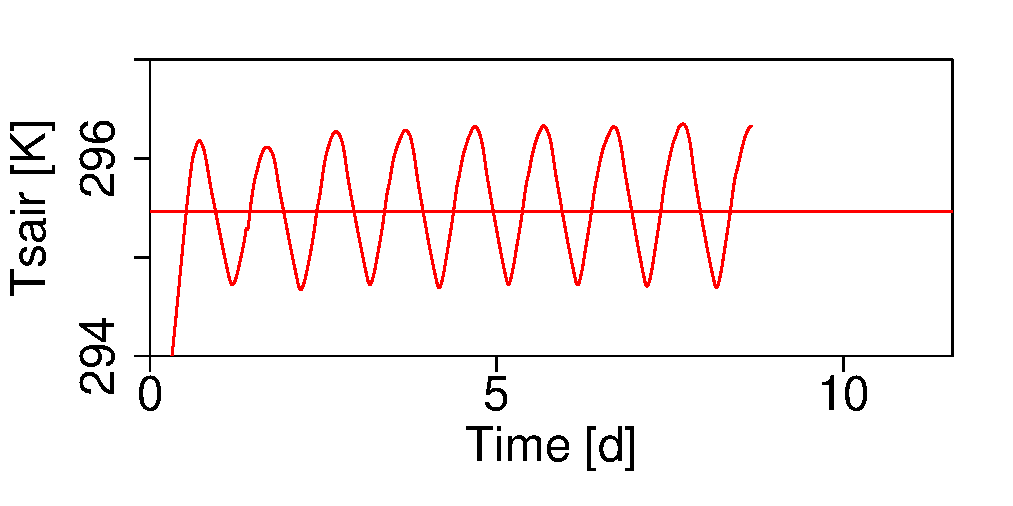
\includegraphics[trim={0 1.35cm 0cm 0}, clip, width=0.45\linewidth]{tsair_T0_300K_ampl_10_1km_timeseries.pdf}}
\put(  30,36){
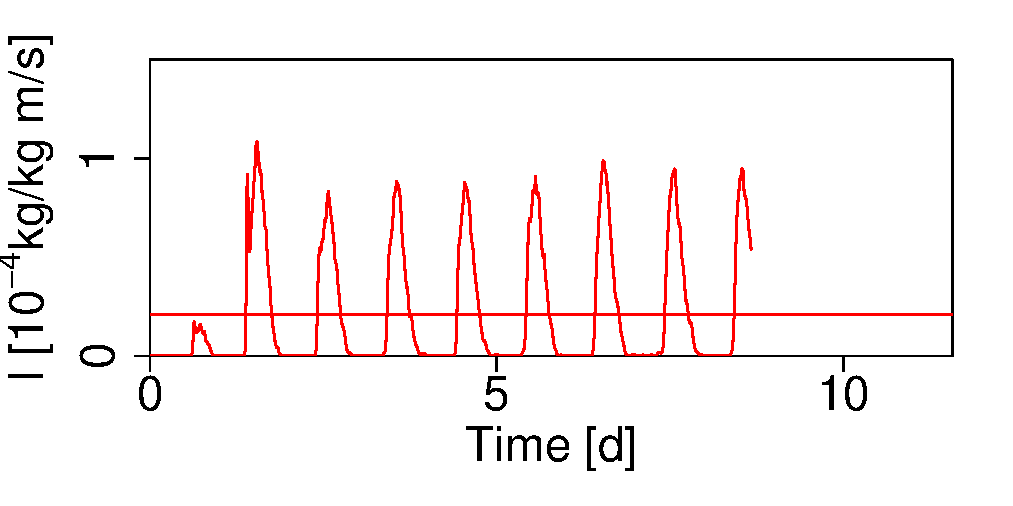
\includegraphics[trim={0 1.35cm 0cm 0}, clip, width=0.45\linewidth]{prcp_T0_300K_ampl_10_1km_timeseries.pdf}}
\put(-55,-1){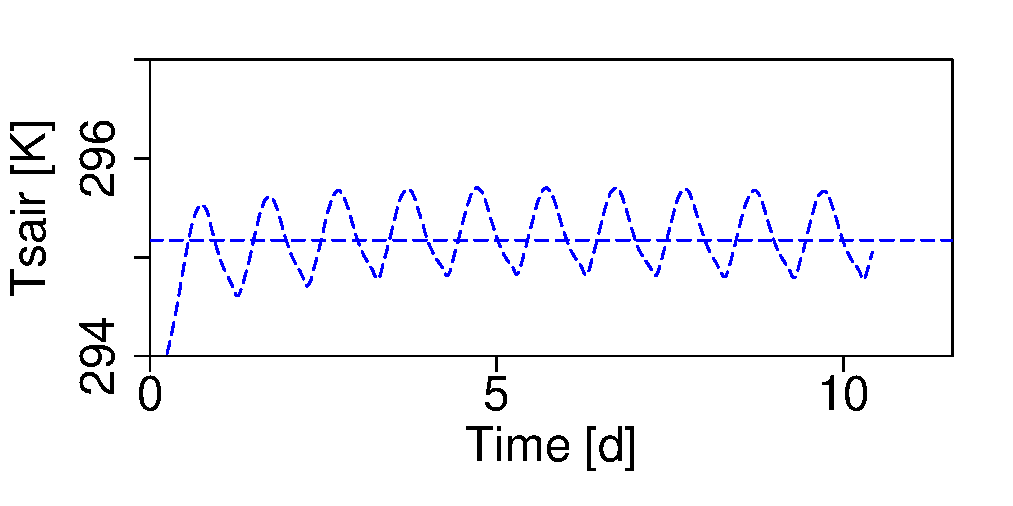
\includegraphics[trim={0 0cm 0cm 0}, clip, width=0.45\linewidth]{tsair_T0_300K_ampl_4_1km_timeseries.pdf}}
\put(  30,-1){
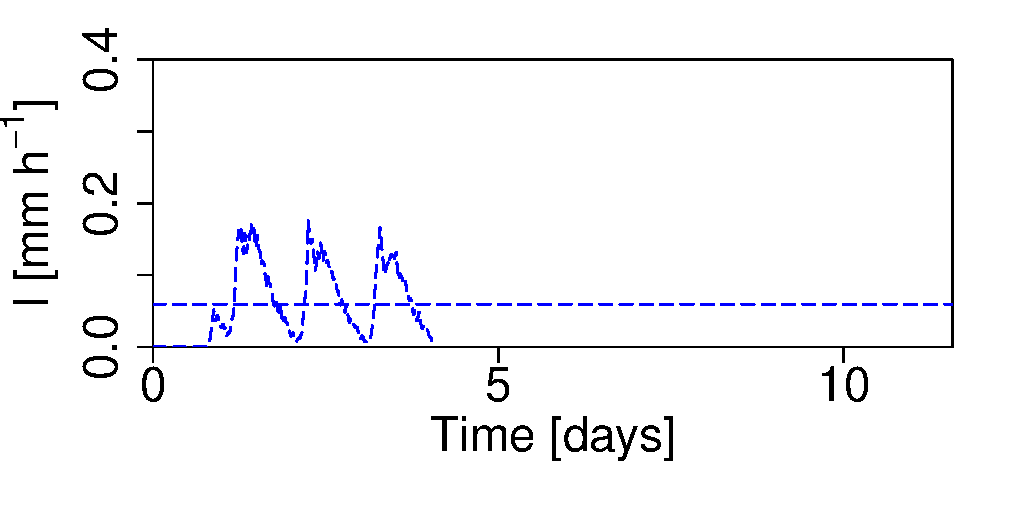
\includegraphics[trim={0 0 0cm 0}, clip, width=0.45\linewidth]{prcp_T0_300K_ampl_4_1km_timeseries.pdf}}
\put(-42,65){\bf a}
\put( 45,65){\bf b}
\put(-42,35){\bf c}
\put( 45,35){\bf d}
%\put( 62,53){\bf c}
\end{overpic}
\caption{{\bf Multi-day timeseries of domain averaged quantities}. 
{\bf a}, Domain-mean near-surface temperature for simulation A5b. The horizontal line indicates the time average over the entire timeseries;
{\bf b}, Analogous to (a), but for rain rate;
{\bd c,d}, Analogous to (a),(b), but for the simulation A2b ({\it compare}: Tab.~\ref{tab:experiments}).
}
\label{fig:multi-day_timeseries}
\end{figure*}


\begin{figure*}[!]
\centering
\begin{overpic}[width=0.4\textwidth ]{dummy.pdf}
\put(-60,0){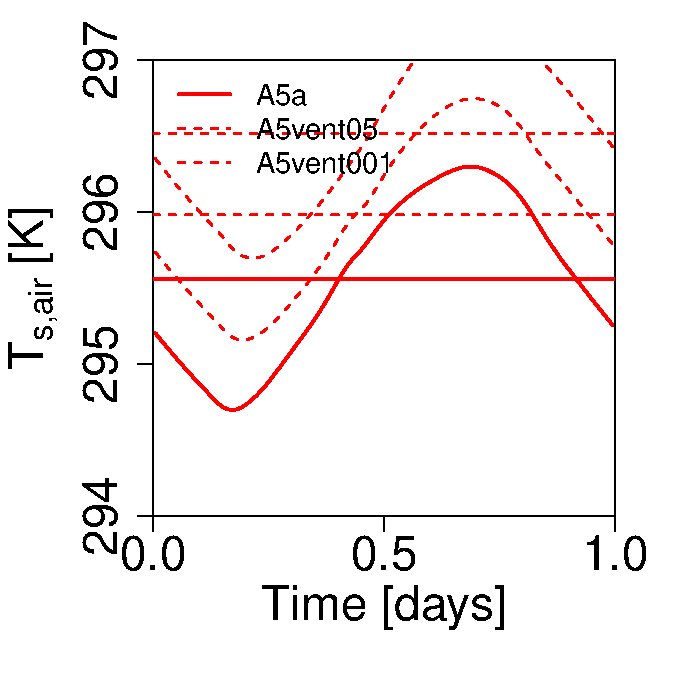
\includegraphics[trim={0 0 0cm 0}, clip, height=0.32\linewidth]{tsair_vent_timeseries_agg.pdf}}
\put(-5,0){
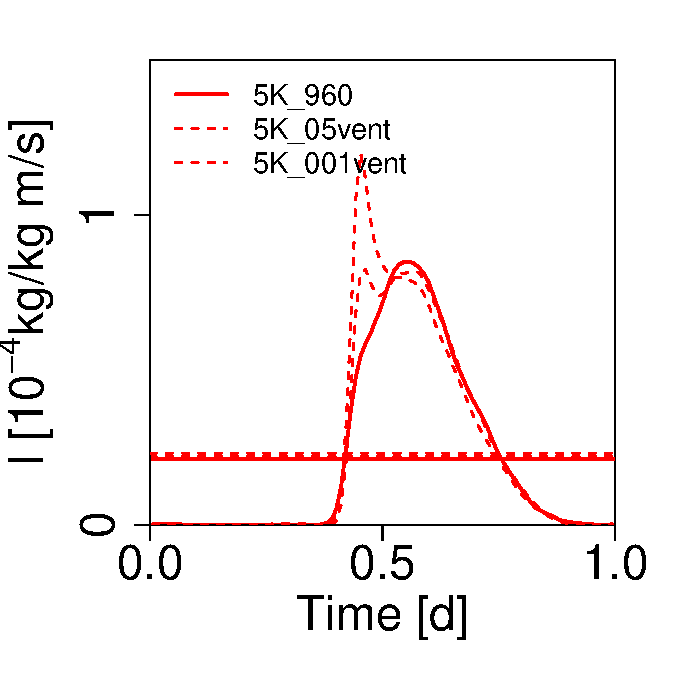
\includegraphics[trim={0 0 0cm 0}, clip, height=0.32\linewidth]{prcp_vent_timeseries_agg.pdf}}
\put(50,0){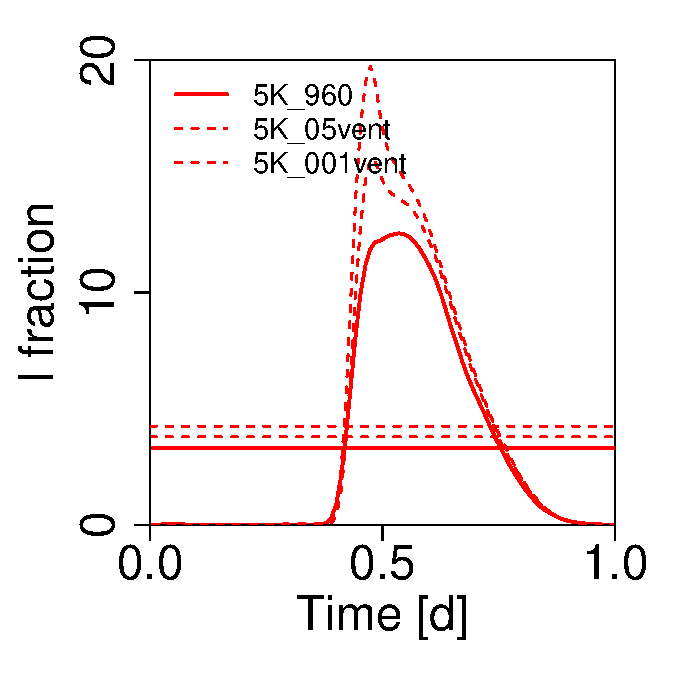
\includegraphics[trim={0 0 0cm 0}, clip, height=0.32\linewidth]{pfrac_vent_timeseries_agg.pdf}}
\put(-45,53){\bf a}
\put( 11,53){\bf b}
\put( 62,53){\bf c}
\end{overpic}
\caption{{\bf Diurnal cycles of domain averaged quantities}. [here we might also want to show $T(6000m)$ and specific humidity.]
Similar to Fig.~\ref{fig:domain_mean_timeseries} but reducing the ventilation coefficient to a fraction of $.5$ and $.01$, respectively. 
}
\label{fig:domain_mean_timeseries_ventilation}
\end{figure*}

\begin{figure*}[!]
\centering
\begin{overpic}[width=0.4\textwidth ]{dummy.pdf}
\put(-60,0){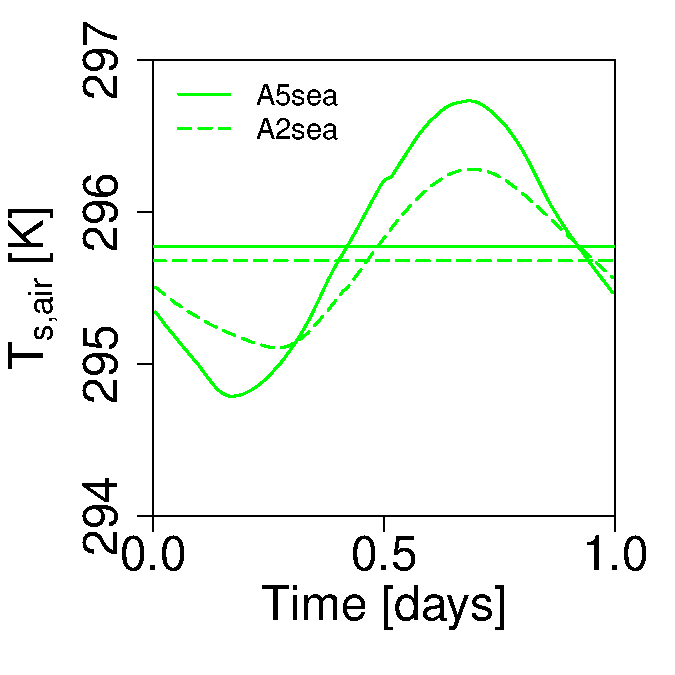
\includegraphics[trim={0 0 0cm 0}, clip, height=0.32\linewidth]{tsair_sea_timeseries_agg.pdf}}
\put(-5,0){
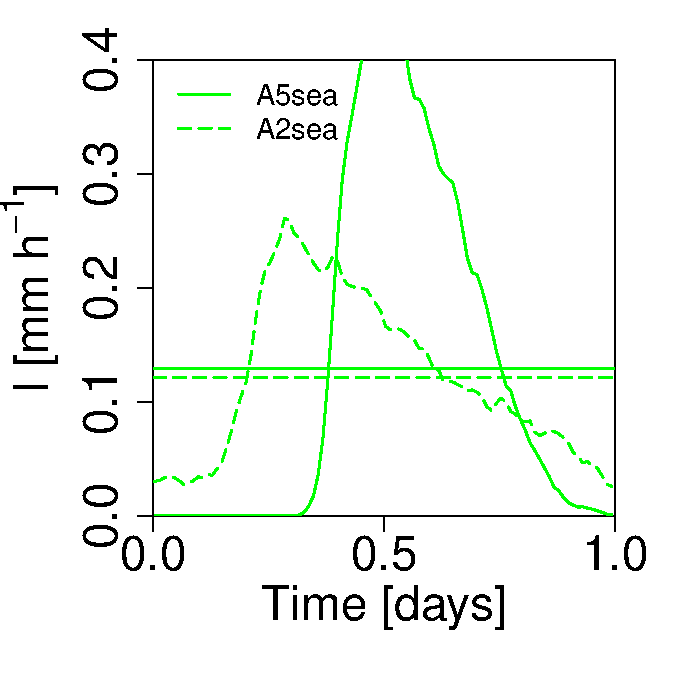
\includegraphics[trim={0 0 0cm 0}, clip, height=0.32\linewidth]{prcp_sea_timeseries_agg.pdf}}
\put(50,0){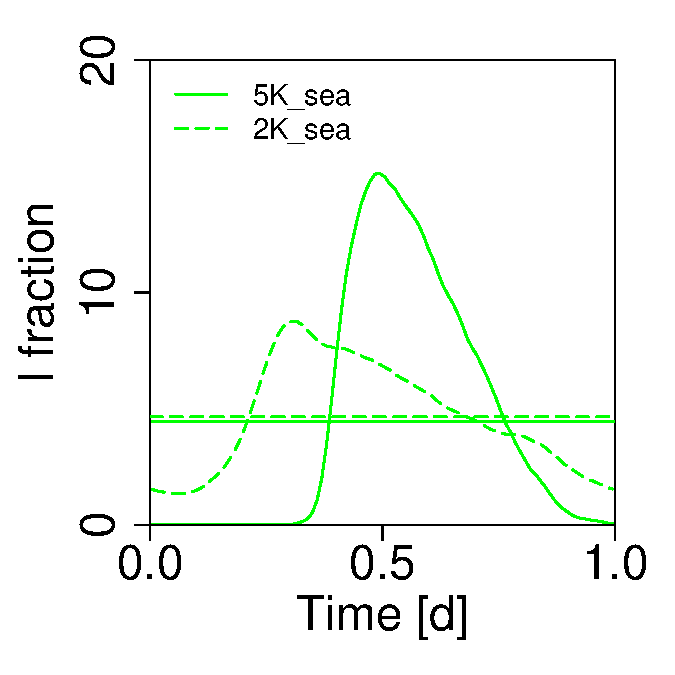
\includegraphics[trim={0 0 0cm 0}, clip, height=0.32\linewidth]{pfrac_sea_timeseries_agg.pdf}}
\put(-45,53){\bf a}
\put( 11,53){\bf b}
\put( 62,53){\bf c}
\end{overpic}
\caption{{\bf Diurnal cycles of domain averaged quantities}. [here we might also want to show $T(6000m)$ and specific humidity.]
Similar to Fig.~\ref{fig:domain_mean_timeseries} but using $100$ percent surface evaporation. 
}
\label{fig:domain_mean_timeseries_surface_evap}
\end{figure*}


\begin{figure*}
\centering
%\begin{overpic}
%\includegraphics[height=0.33\linewidth]{cavities}
\centering
\begin{overpic}[width=0.4\textwidth ]{dummy.pdf}
\put(-55,0){
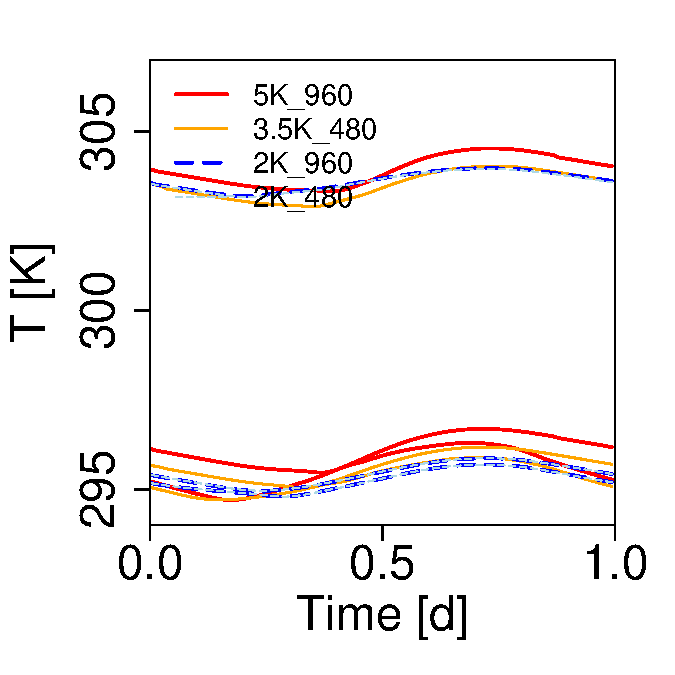
\includegraphics[trim={0 0 0cm 0}, clip, height=0.32\linewidth]{t_varying_ampl_timeseries_agg_p.pdf}}
\put(0,0){
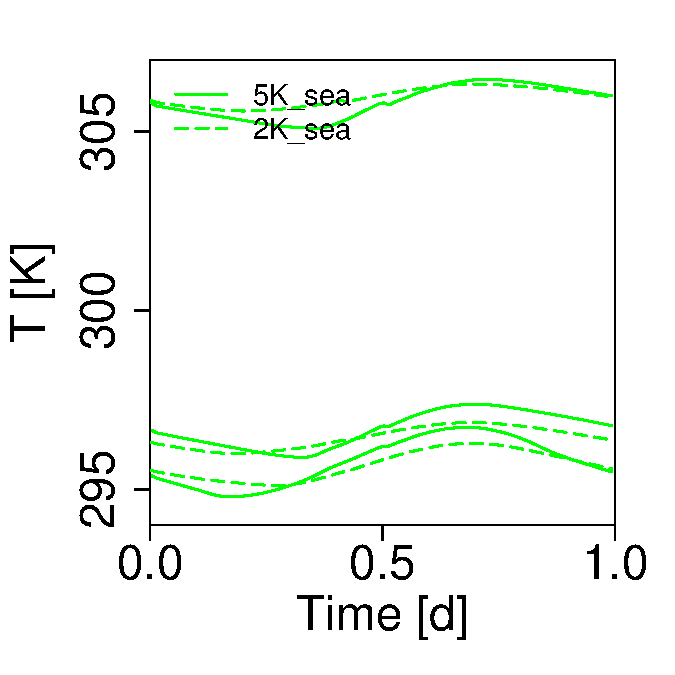
\includegraphics[trim={0cm 0 0cm 0}, clip, height=0.32\linewidth]{t_sea_timeseries_agg_p.pdf}}
\put(55,0){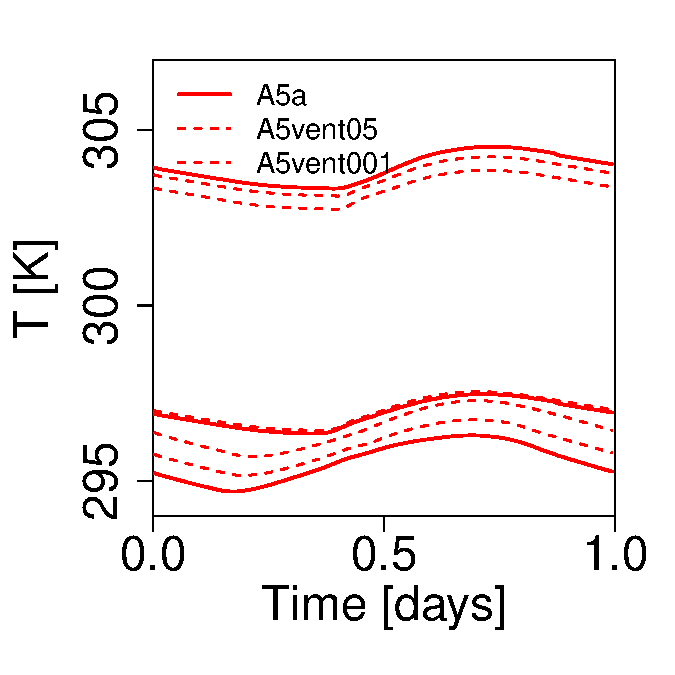
\includegraphics[trim={0cm 0 0cm 0}, clip, height=0.32\linewidth]{t_vent_timeseries_agg_p.pdf}}
\put(-42,53){\bf a}
\put( 14,53){\bf b}
\put( 67,53){\bf c}
\end{overpic}
\caption{{\bf Diurnal cycles of surface and free troposphere temperature}. [here we might also want to show $T(6000m)$ and specific humidity.]
As in Fig.~\ref{fig:domain_mean_timeseries}a, but including free-tropospheric temperature [add the exact height when ready].
{\bf a}, Varying forcing amplitude $T_a$;
{\bf b}, Similar, but for sea surface conditions;
{\bf c}, Varying the ventilation coefficient.
}
\label{fig:free_trop_temp}
\end{figure*}

\begin{figure*}
\centering
%\begin{overpic}
%\includegraphics[height=0.33\linewidth]{cavities}
\centering
\begin{overpic}[width=0.4\textwidth ]{dummy.pdf}
\put(-55,0){
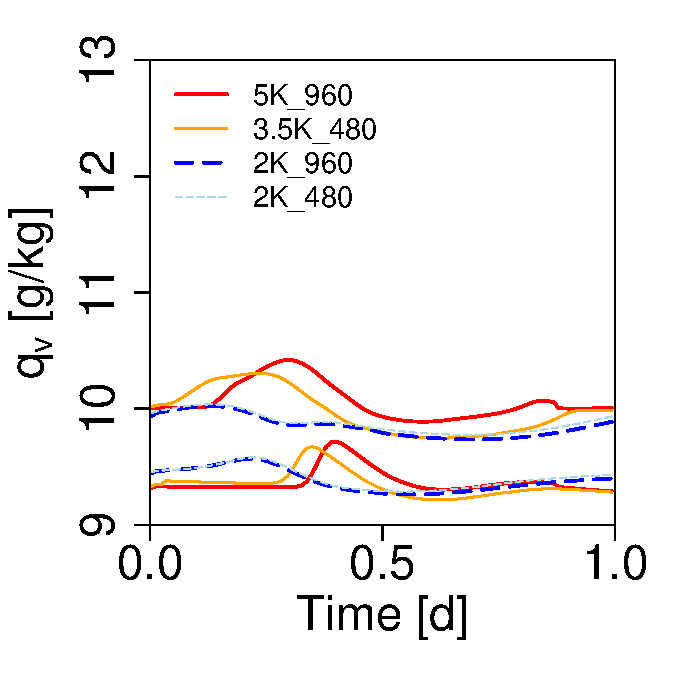
\includegraphics[trim={0 0 0cm 0}, clip, height=0.32\linewidth]{q_varying_ampl_timeseries_agg_p.pdf}}
\put(0,0){
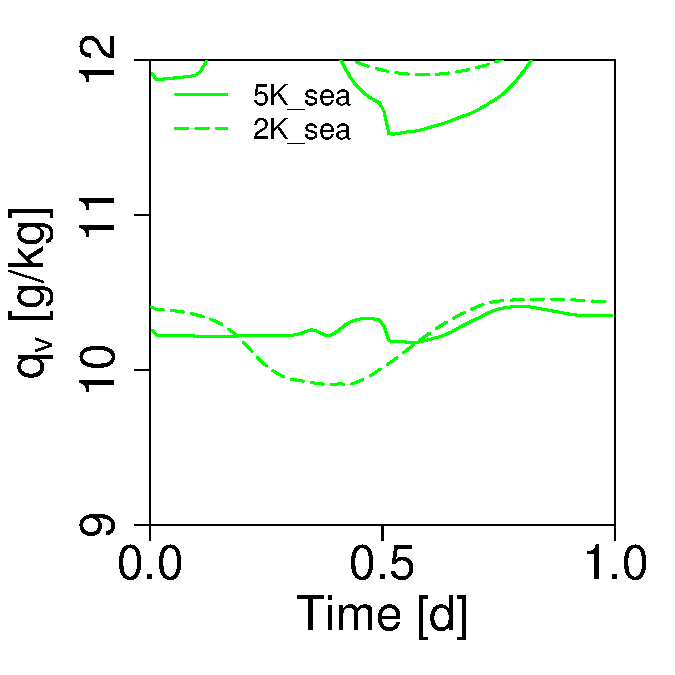
\includegraphics[trim={0cm 0 0cm 0}, clip, height=0.32\linewidth]{q_sea_timeseries_agg_p.pdf}}
\put(55,0){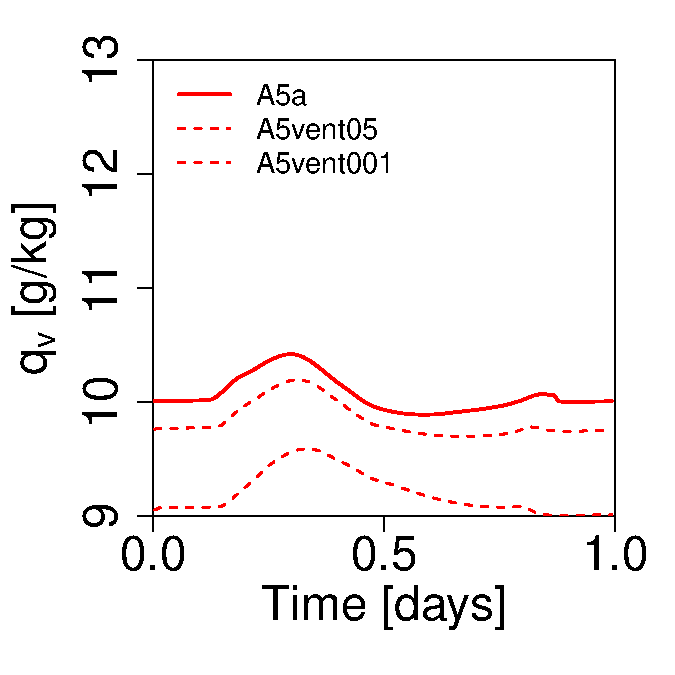
\includegraphics[trim={0cm 0 0cm 0}, clip, height=0.32\linewidth]{q_vent_timeseries_agg_p.pdf}}
\put(-42,53){\bf a}
\put( 14,53){\bf b}
\put( 67,53){\bf c}
\end{overpic}
\caption{{\bf Diurnal cycles of surface and free troposphere specific humidity}. 
As in Fig.~\ref{fig:free_trop_temp}, but for free-tropospheric specific humidity [add the exact height when ready].
}
\label{fig:humidity}
\end{figure*}



\begin{figure}
\centering
%\begin{overpic}
%\includegraphics[height=0.33\linewidth]{cavities}
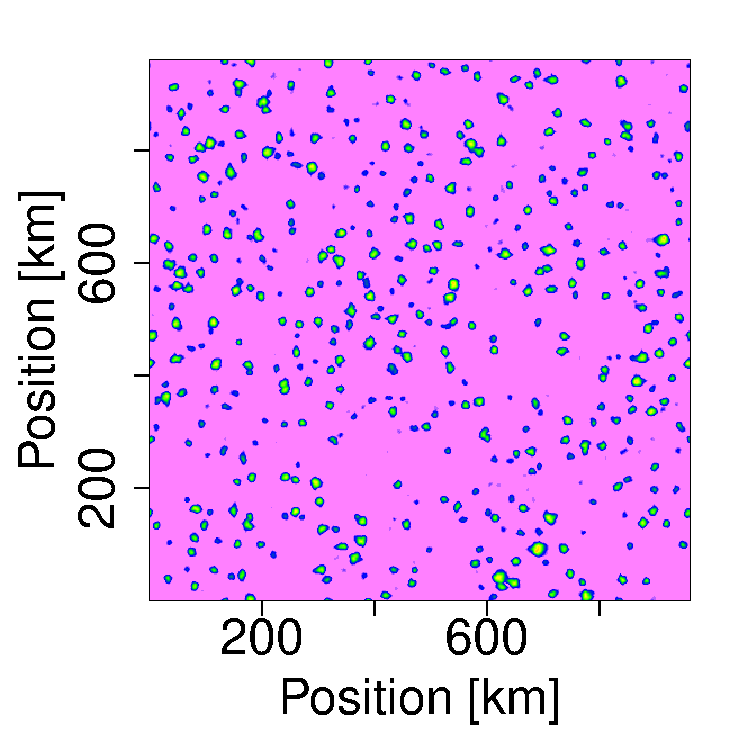
\includegraphics[trim={2cm 2.4cm 1cm 1cm}, clip, height=0.11\linewidth]{1-288_T0_300K_ampl_10_500m_r_int_timmean_xy_plot_l=2.pdf}
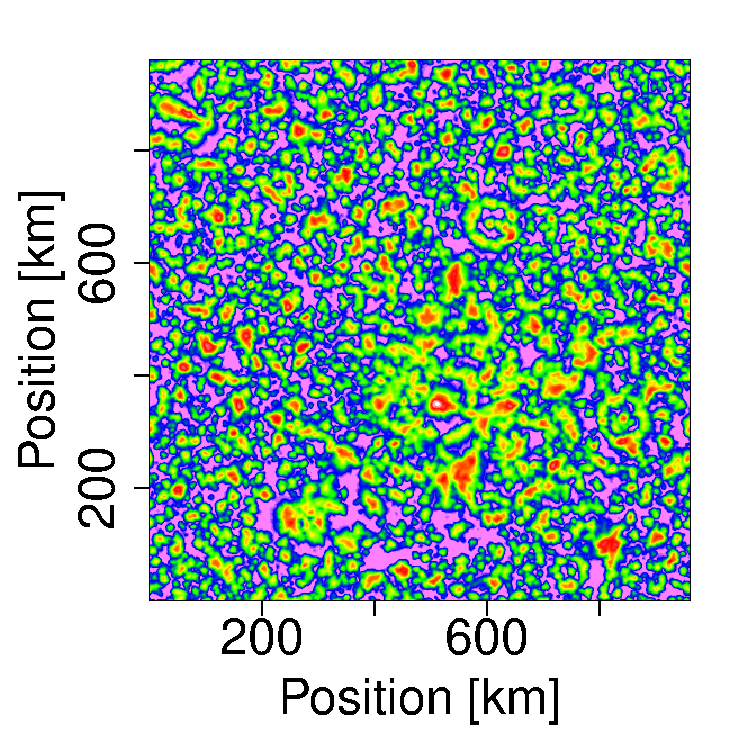
\includegraphics[trim={2cm 2.4cm 1cm 1cm}, clip, height=0.11\linewidth]{289-576_T0_300K_ampl_10_500m_r_int_timmean_xy_plot_l=2.pdf}
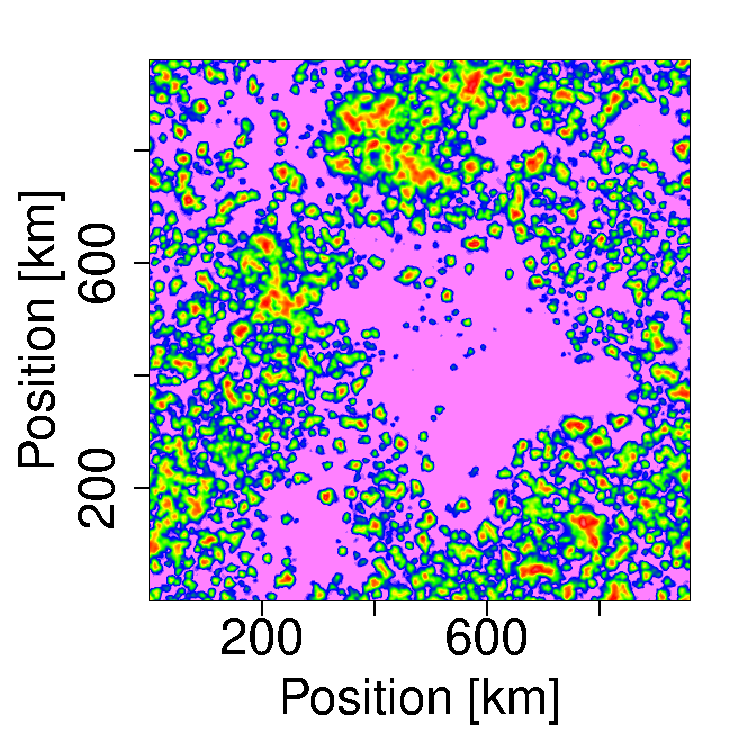
\includegraphics[trim={2cm 2.4cm 1cm 1cm}, clip, height=0.11\linewidth]{577-864_T0_300K_ampl_10_500m_r_int_timmean_xy_plot_l=2.pdf}
\caption{{\bf Daily precipitation sum for higher lateral model resolution.}. }
\label{fig:daily_sum_500m}
\end{figure}


\end{document}

